\mode*
\begin{frame}[label=motivacion]
  \motivacionTime
  \frametitle{Por qu\'e esta investigaci\'on?}
  \framesubtitle{Algunos aspecto para la justificaci\'on}
  \quad\hspace{-0.8cm}\vspace{-0.5cm}
  \begin{columns}[T,totalwidth=0.97\textwidth]
    \small
    \begin{column}{0.55\textwidth}\setbeamercovered{transparent}
      \begin{enumerate}
      \item<1-|alert@1|uncover@1-6> Como ayuda de la proliferaci\'on
        \only<2-6>{
          \textit{\textbf{Ejemplo proceso de dise\~no:}}\setbeamercovered{transparent}
          \begin{itemize}\scriptsize
          \item<2-|alert@2|uncover@2> Bajo costo
          \item<3-|alert@3|uncover@3> Didacticos
          \item<4-|alert@4|uncover@4> Modularidad
          \item<5-|alert@5|uncover@5> Prototipado rapido
          \item<6-|alert@6|uncover@6> Metodologia de dise\~no
          \end{itemize}
        }
      \item<7-|alert@7|uncover@7-8> Motivaci\'on personal
      \item<9-|alert@9|uncover@9-19> Posibles productos y soluciones
        \only<9-19>{
          \begin{itemize}\scriptsize
            \setbeamercovered{transparent}
          \item<10-|alert@10|uncover@10-11> Teleoperaci\'on
          \item<12-|alert@12|uncover@12-13> Manufactura, transporte y ensambles
          \item<14-|alert@14|uncover@14-15> Movilidad en cuadrapl\'ejicos, pr\'otesis y caminata pasiva
          \item<16-|alert@16|uncover@16-17> Educaci\'on, cursos y materias
          \item<18-|alert@18|uncover@18-19> Entretenimiento e IA
          \end{itemize}
        }
      \item<20-|alert@20|uncover@20-32> Viabilidad
        \only<21-32>{
          \begin{itemize}\scriptsize\setbeamercovered{transparent}
          \item<21-|alert@21|uncover@21-22> Recursos f\'isicos
          \item<23-|alert@23|uncover@23-24> Profesores, grupos de investigaci\'on y materias
          \item<25-|alert@25|uncover@25-26> Convocatorias para recursos econ\'omicos y financiaci\'on
          \item<27-|alert@27|uncover@27-28> Relaciones con grupos internacionales de investigaci\'on
          \item<29-|alert@29|uncover@29-30> Experiencia del director de investigaci\'on en el tema
          \item<31-|alert@31|uncover@31-32> Experiencia del investigador en el tema del proyecto
          \end{itemize}
        }
      \item<33-|alert@33|uncover@33-38> Posible pasant\'ia
        \begin{itemize}\scriptsize
        \item<34-|alert@34|uncover@34> KUKA ROBOTICS
        \item<35-|alert@35|uncover@35> DLR-biped
        \item<36-|alert@36|uncover@36> Profesor M\'aximo Roa
        \item<37-|alert@37|uncover@37> Proyecto reciente
        \item<38-|alert@38|uncover@38> L\'ineas sugeridas de investigaci\'on
        \end{itemize}
      \end{enumerate}
    \end{column}
    \begin{column}{0.4\textwidth}
      \parbox[c][7cm][c]{4.0cm}{
        \only<1-4>{
          \begin{center}
            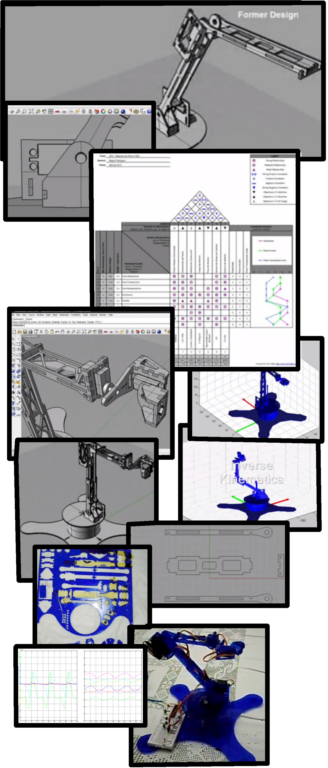
\includegraphics[height=7cm]{../images/RobotMR1_0.png}
          \end{center}
        }
        \only<5>{
          % 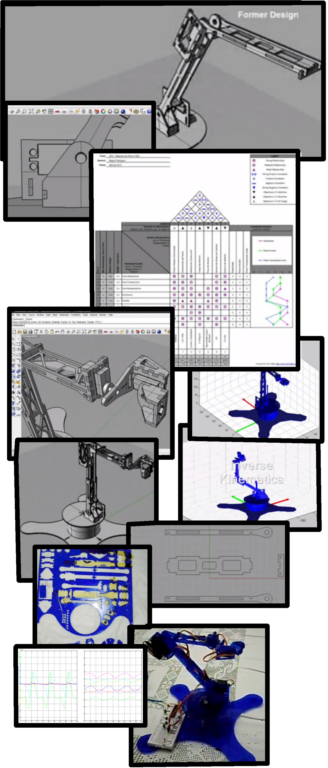
\includegraphics[height=7cm]{../images/RobotMR1_0.png}
          \begin{center}
            \animategraphics[height=7cm,autoresume,autoplay]{3}{../images/RobotMR1_}{0}{12}
          \end{center}
        }
        \only<6>{
          \begin{center}
            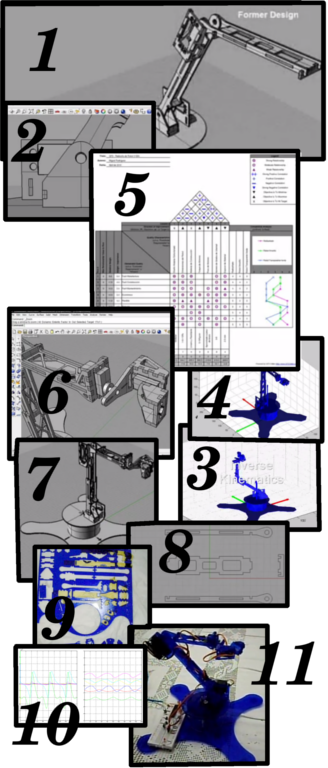
\includegraphics[height=7cm]{../images/RobotMR1_12.png}
          \end{center}
          % \movie[width=3cm,height=7cm,externalviewer]{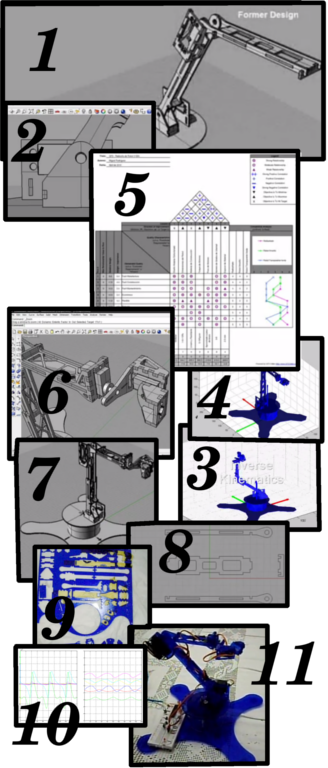
\includegraphics[height=7cm]{../images/RobotMR1_12.png}}{../videos/RobotMR1.flv} 
        }
        \only<8>{
          \begin{center}
            \animategraphics[height=7cm,autoresume,autoplay]{2}{../images/SomeThingsByMeSumary_}{0}{4}
            % 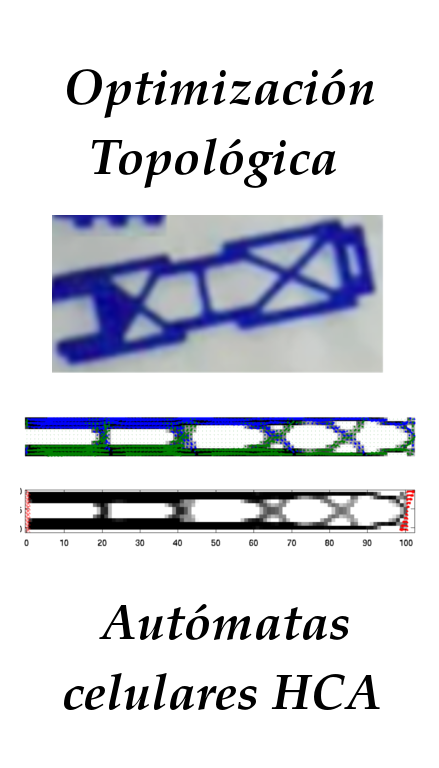
\includegraphics[height=7.0cm]{../images/SomeThingsByMeSumary_0.png}
          \end{center}
        }
        \only<11>{
          \begin{center}
            \textbf{\textcolor{redun}{Teleoperaci\'on}}\\[0.3cm]
            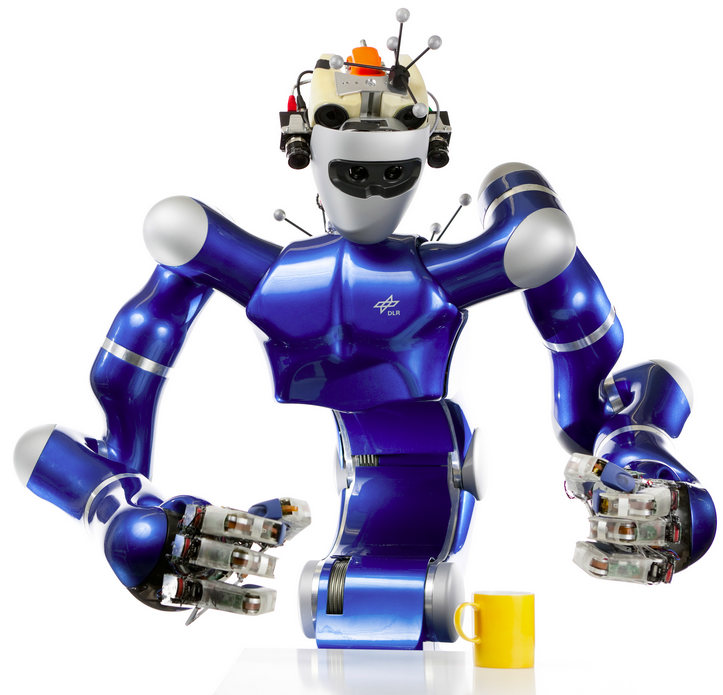
\includegraphics[width=4.0cm]{../images/Teleoperacion.png}
          \end{center}
        }
        \only<13>{
          \begin{center}
            \textbf{\textcolor{redun}{Transporte}}\\[0.3cm]
            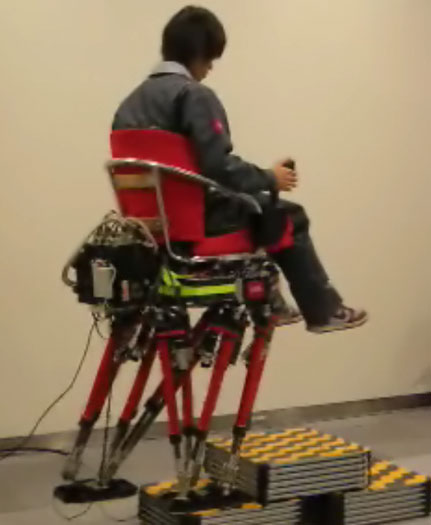
\includegraphics[width=4.0cm]{../images/Transporte.png}
          \end{center}
        }
        \only<15>{
          \begin{center}
            \textbf{\textcolor{redun}{Biomec\'anica}}\\[0.3cm]
            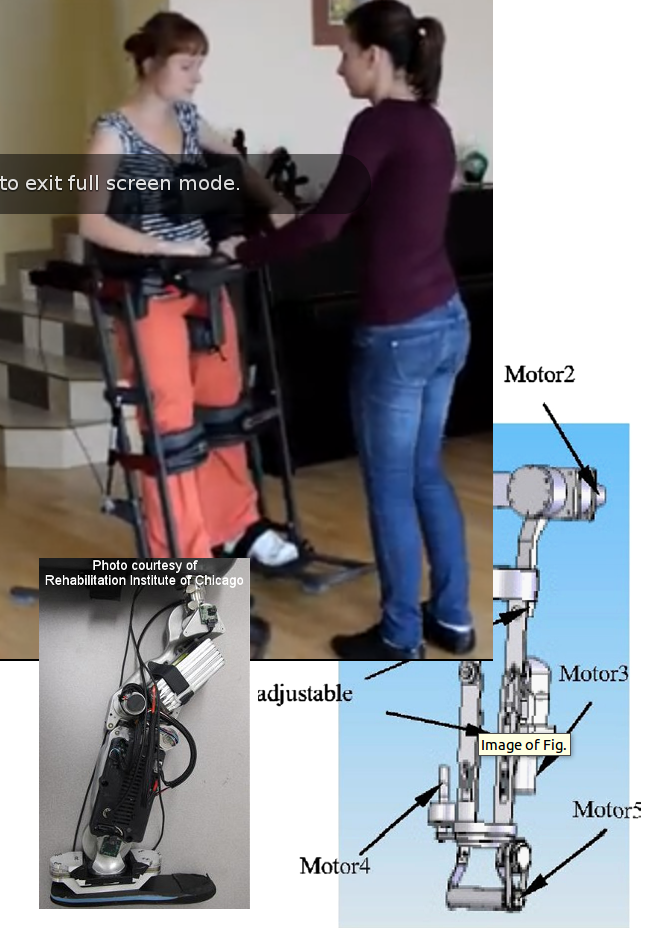
\includegraphics[width=4.0cm]{../images/ProsthesisAndPhysiotherapy.png}
          \end{center}
        }
        \only<17>{
          \begin{center}
            \textbf{\textcolor{redun}{Educaci\'on}}\\[0.3cm]
            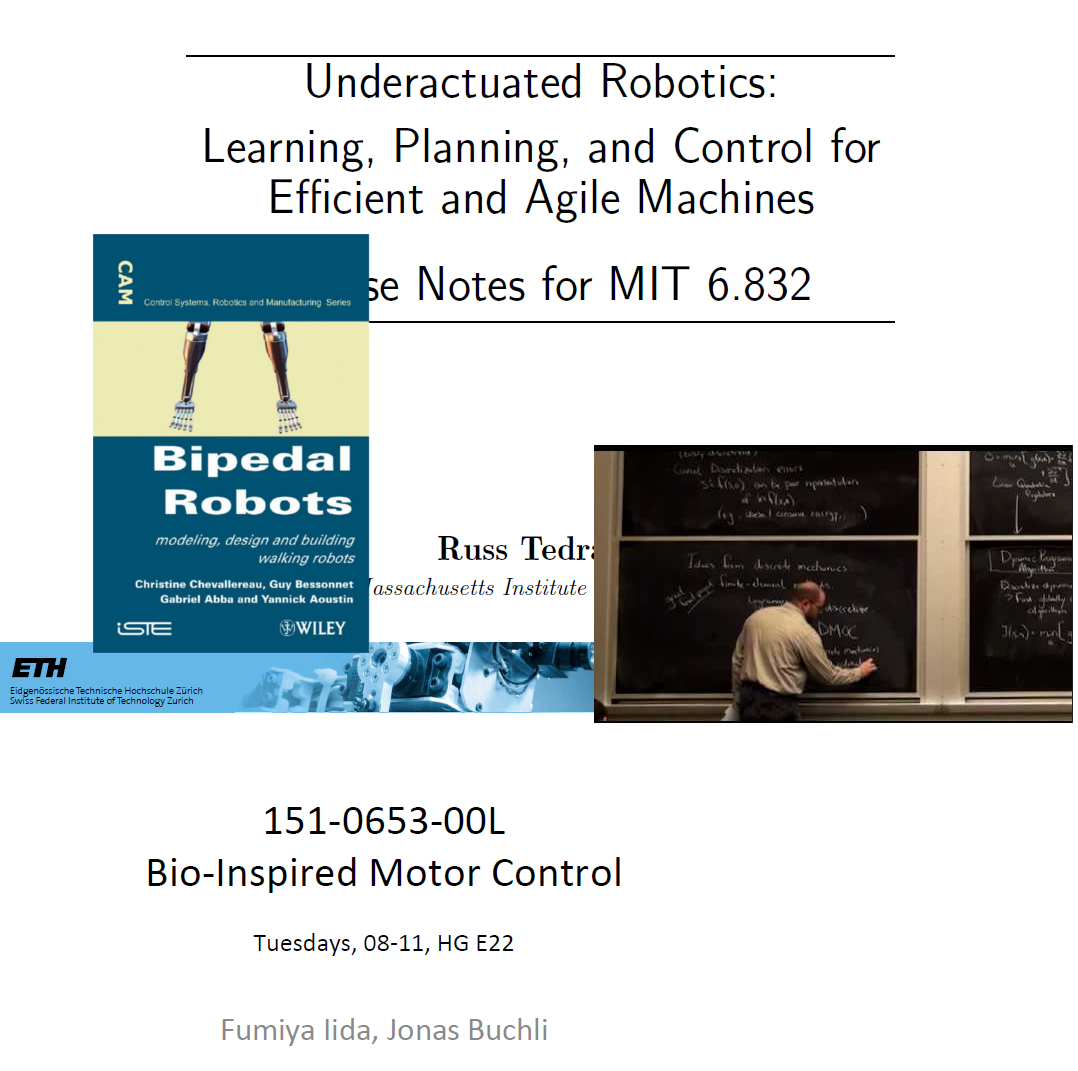
\includegraphics[width=4.0cm]{../images/Educacion.png}
          \end{center}
        }
        \only<19>{
          \begin{center}
            \textbf{\textcolor{redun}{Entretenimiento}}\\[0.3cm]
            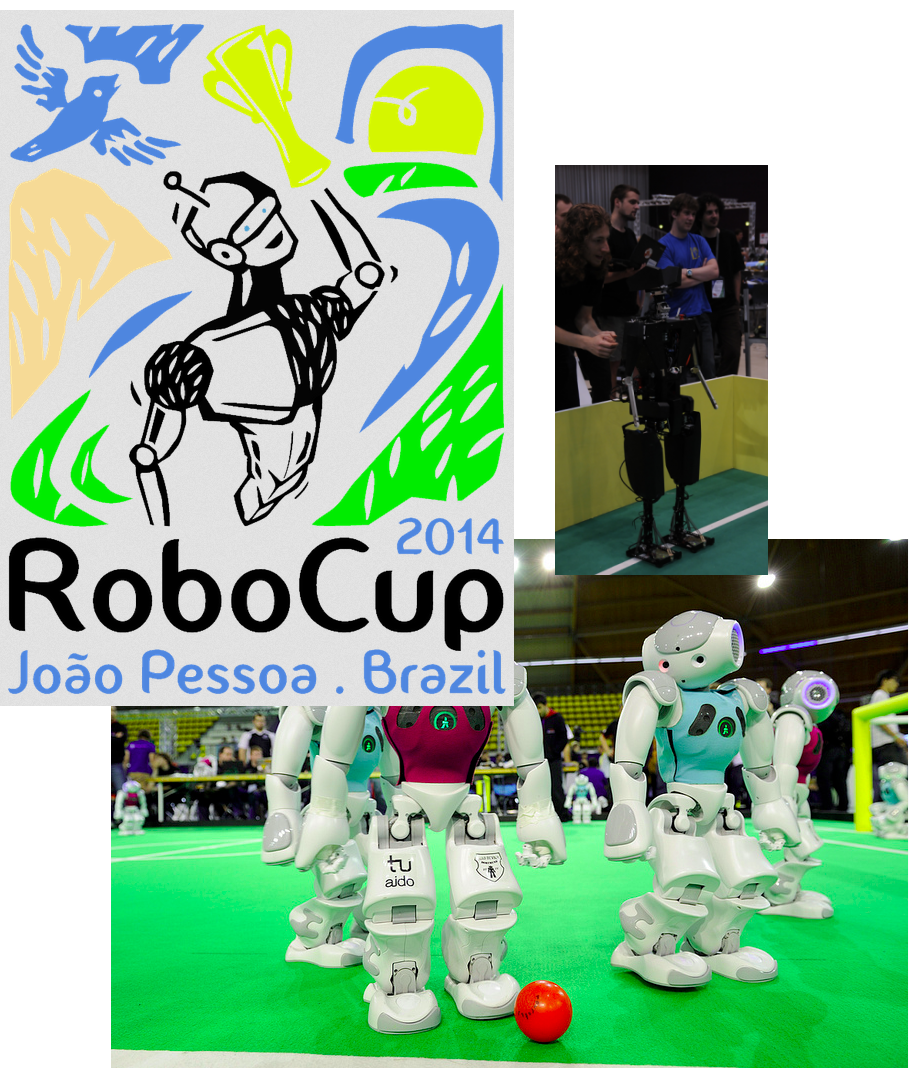
\includegraphics[width=4.0cm]{../images/Entretenimiento.png}
          \end{center}
        }
        \only<22>{
          \begin{center}
            \textbf{\textcolor{redun}{Recursos Disponibles}}
            \begin{itemize}\scriptsize
            \item CNC
            \item Impresoras 3D
            \item Software CAD-CAM-CAE
            \item Laboratorios con plataformas
            \end{itemize}
          \end{center}
        }
        \only<24>{
          \begin{center}
            \textbf{\textcolor{redun}{Lista de profesores}}
            \begin{enumerate}\tiny
            \item Din\'amica de robots\\{\tiny(R. Ram\'irez)}
            \item Biomec\'anica\\{\tiny(D. Garzon)}
            \item Sistemas embebidos\\{\tiny(C. Camargo)}
            \item Control de robots\\{\tiny(J. Sofrony)}
            \item Computaci\'on flexible\\{\tiny(V.H Grisales)}
            \item Aprendizaje de m\'aquina\\{\tiny(F. Gonz\'alez)}
            \item Optimizaci\'on\\{\tiny(A. Guzman)}
            \item Computaci\'on flexible\\{\tiny(L.F Ni\~no)}
            \item Inteligencia Artificial\\{\tiny(J. G\'omez)}
            \end{enumerate}
          \end{center}
        }
        \only<26>{
          \begin{center}
            \textbf{\textcolor{redun}{Convocatorias}}
            \begin{itemize}\scriptsize
            \item DIB
            \item VRi
            \item Colciencias
            \item Col-CAPES
            \item Col-DAAD
            \item Otras
            \end{itemize}
          \end{center}
        }
        \only<28>{
          \begin{center}
            \textbf{\textcolor{redun}{Posibles Relaciones}}
            \scriptsize
            \begin{itemize}
            \item Justin DLR (M. Roa)
            \item Robonaut 2 GM-NASA (L. Barajas)
            \item Walking Dynamics Conferences
            \item Clawar Conferences
            \end{itemize}
          \end{center}
        }
        \only<30>{
          \begin{center}
            \animategraphics[height=7cm,autoresume,autoplay]{1}{../images/SomeThingsByRR_}{0}{2}
            % 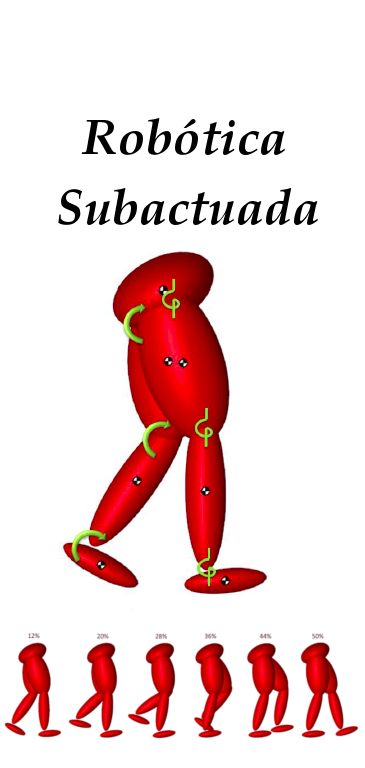
\includegraphics[height=7.0cm]{../images/SomeThingsByRR_0.png}
          \end{center}
        }
        \only<32>{
          \scriptsize
          \begin{center}%P1(120,360),P2(1110,530)
            % \includegraphics[height=7cm]{../images/SomeThingsByMe_0.png}
            \animategraphics[height=7cm,autoresume,autoplay]{1.5}{../images/SomeThingsByMe_}{1}{5}
          \end{center}
        }
        \only<33-38>{
          \scriptsize
          \begin{center}%P1(120,360),P2(1110,530)
            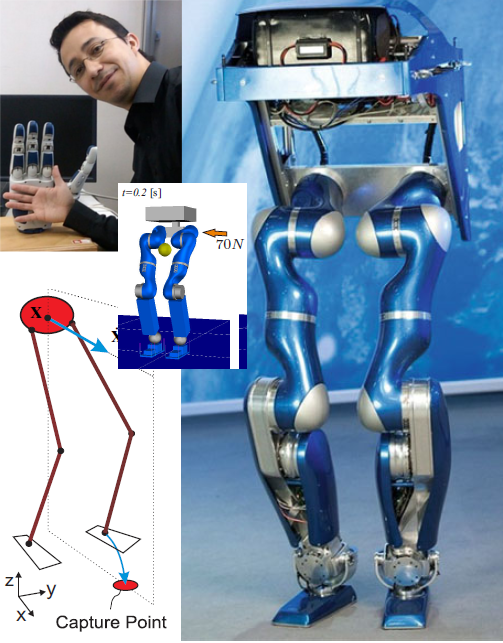
\includegraphics[width=4cm]{../images/DLR-Roa-Tendencias.png}
          \end{center}
        }
      }
    \end{column}
  \end{columns}
  \only<28>{\vspace{-3.5cm}
    \begin{center}
      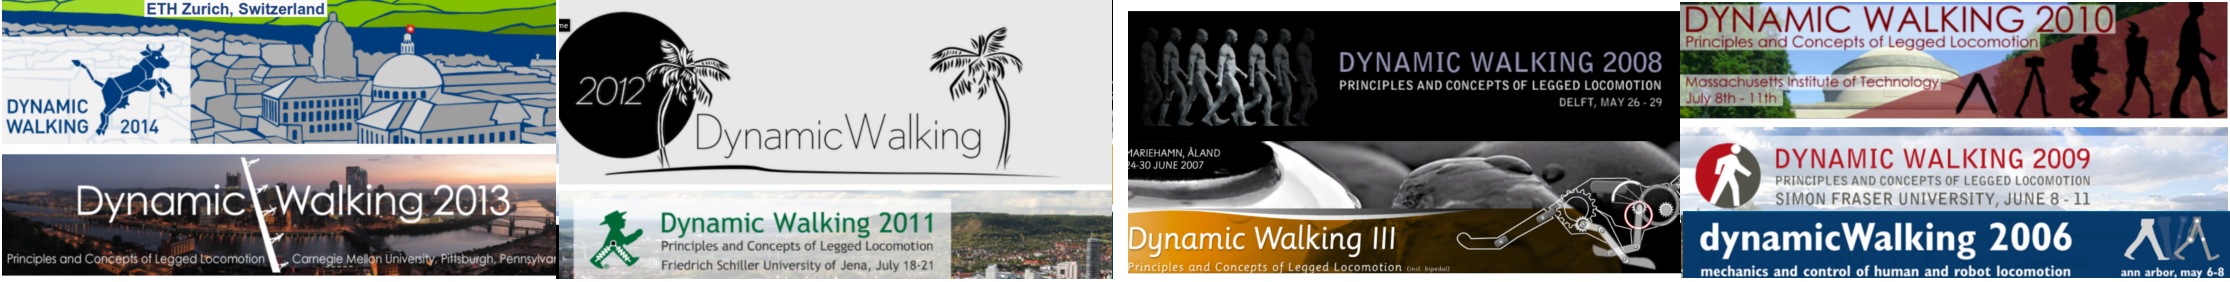
\includegraphics[width=0.95\textwidth]{../images/DynamicWalkingConferences.png}
    \end{center}
  }
\end{frame}
